\documentclass{article}

\usepackage{graphicx}
\usepackage{tikz}
\usepackage{tikzsymbols}
\usetikzlibrary{calc,patterns,shapes.geometric}
\pagestyle{empty}
\usepackage[margin=0pt]{geometry}
\geometry{papersize={14in,12in}}

\def\centerarc[#1](#2)(#3:#4:#5){\draw[#1] ($(#2)+({#5*cos(#3)},{#5*sin(#3)})$) arc (#3:#4:#5);}

\begin{document}
	\begin{figure}
		\centering
		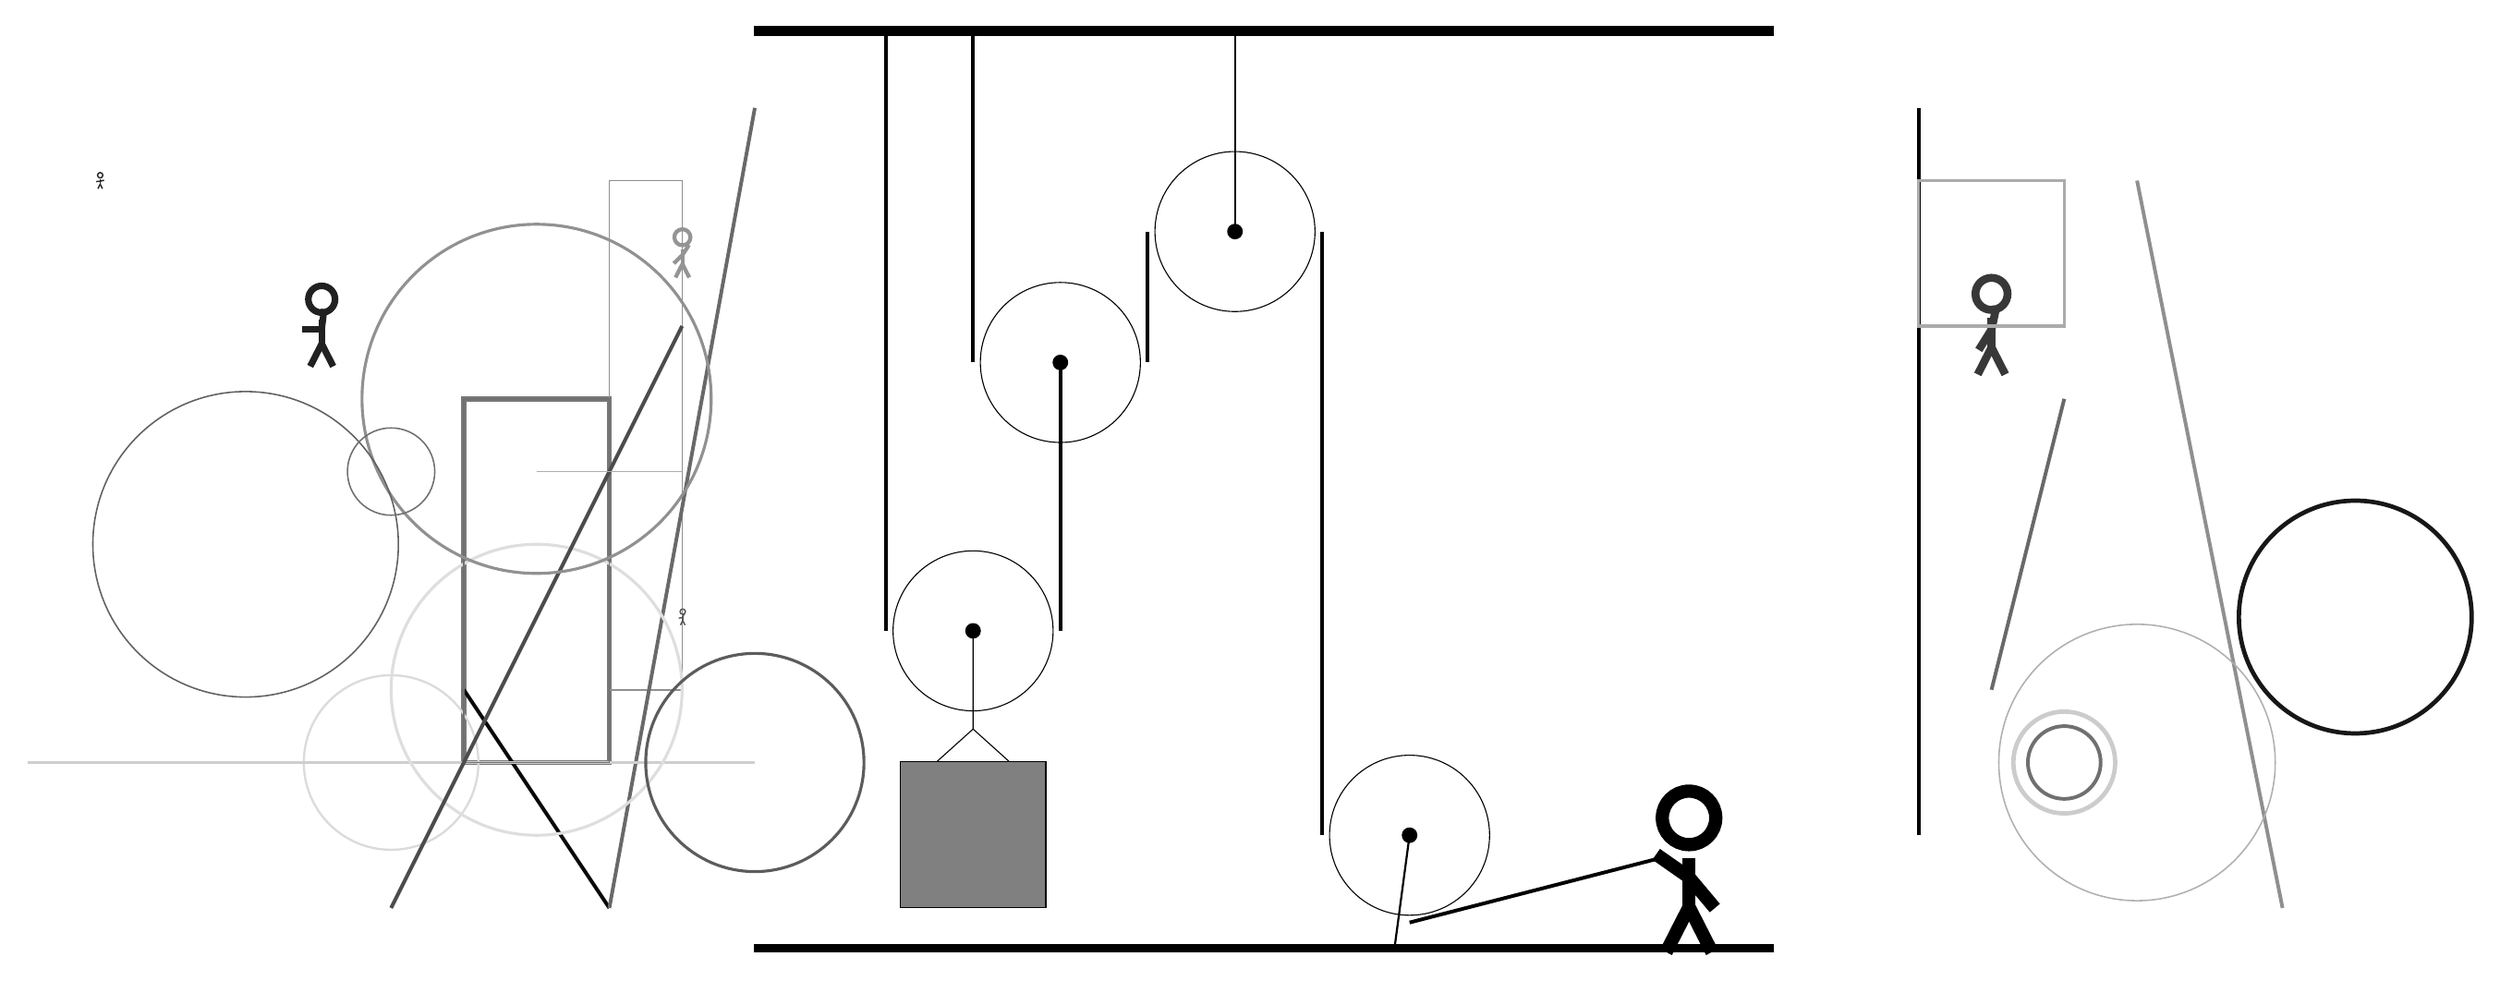
\begin{tikzpicture}
			%%%%% START %%%%%
			
			\draw[fill=black] (-2, 9) rectangle (12, 9.125);
			
			\draw (1, 0.81) circle (1.1);
			\draw[fill=black] (1, 0.81) circle (0.1);
			
			\draw (2.2, 4.5) circle (1.1);
			\draw[fill=black] (2.2, 4.5) circle (0.1);
			
			\draw (4.6, 6.3) circle (1.1);
			\draw[fill=black] (4.6, 6.3) circle (0.1);
			\draw[thick] (4.6, 6.3) -- (4.6, 9);
			
			\draw[line width=0.7mm, color=black!53] (-4, 4) rectangle (-6, -1);
			
			\draw[line width=0.5mm, color=black!100](14, 8) -- (14, -2);
			\draw[line width=0.5mm, color=black!97](-6, 0) -- (-4, -3);
			\draw [line width=0.3mm, color=black!14](-7, -1) circle (1.2);
			
			\draw[line width=0.2mm, color=black!44] (-3, 0) rectangle (-4, 7);
			\draw[line width=0.5mm, color=black!59](-4, -3) -- (-2, 8);
			\draw[line width=0.5mm, color=black!19](-2, -1) -- (-12, -1);
			\draw [line width=0.4mm, color=black!13](-5, 0) circle (2.0);
			\draw[line width=0.5mm, color=black!59](16, 4) -- (15, 0);
			\draw[line width=0.2mm, color=black!56] (-4, 4) rectangle (-6, -1);
			\draw[line width=0.5mm, color=black!70](-3, 5) -- (-7, -3);
			\draw [line width=0.6mm, color=black!20](16, -1) circle (0.7);
			\node[line width=0.5mm, color=black!87] at (-8, 5) {\Strichmaxerl[5][0][83]};
			
			\draw [line width=0.6mm, color=black!91](20, 1) circle (1.6);
			\draw[line width=0.5mm, color=black!44](17, 7) -- (19, -3);
			\node[line width=0.2mm, color=black!67] at (-3, 1) {\Strichmaxerl[1][7][71]};
			
			\draw [line width=0.2mm, color=black!31](17, -1) circle (1.9);
			\draw [line width=0.4mm, color=black!43](-5, 4) circle (2.4);
			\node[line width=0.5mm, color=black!78] at (15, 5) {\Strichmaxerl[6][58][78]};
			\draw [line width=0.4mm, color=black!64](-2, -1) circle (1.5);
			\draw [line width=0.2mm, color=black!62](-9, 2) circle (2.1);
			
			\node[line width=0.3mm, color=black!86] at (-11, 7) {\Strichmaxerl[1][5][14]};
			\draw[line width=0.4mm, color=black!33] (14, 5) rectangle (16, 7);
			\draw [line width=0.2mm, color=black!56](-7, 3) circle (0.6);
			\node[line width=0.4mm, color=black!42] at (-3, 6) {\Strichmaxerl[3][44][57]};
			
			\draw[line width=0.2mm, color=black!32] (-3, 3) rectangle (-5, 3);
			\draw [line width=0.5mm, color=black!56](16, -1) circle (0.5);
			
			\draw (7.0, -2) circle (1.1);
			\draw[fill=black] (7.0, -2) circle (0.1);
			\draw[thick] (7.0, -2) -- (6.8, -3.5);
			
			\draw (1, 0.81) -- (1, -0.54) -- (0.5, -0.99) -- (1.5, -0.99) -- (1, -0.54);
			\draw[fill=black!50] (0, -0.99) rectangle (2, -2.99);
			\draw[line width=0.5mm] (-0.2, 9) -- (-0.2, 0.81);
			\centerarc[line width=0.5mm](1, 0.81)(180:360:1.2000000000000002);
			\draw[line width=0.5mm](2.2, 0.81) -- (2.2, 4.5);
			\draw[line width=0.5mm] (1.0, 9) -- (1.0, 4.5);
			\centerarc[line width=0.5mm](2.2, 4.5)(180:360:1.2000000000000002);
			\draw[line width=0.5mm](3.4, 4.5) -- (3.4, 6.3);
			\centerarc[line width=0.5mm](4.6, 6.3)(0:180:1.2000000000000002);
			\draw[line width=0.5mm] (5.8, 6.3) -- (5.8, -2);
			\centerarc[line width=0.5mm](7.0, -2)(0:90:-1.2000000000000002);
			\draw[line width=0.5mm](7.0, -3.2) -- (10.5, -2.3);
			
			\node at (10.8, -2.5) {\Strichmaxerl[10][-35][-50]};
			
			\draw[fill=black] (-2, -3.5) rectangle (12, -3.6);
			
			%%%%% END %%%%%
		\end{tikzpicture}
	\end{figure}	
\end{document}